%!TEX ROOT=../ctutest.tex

\chapter{State of the Art}
%--- FIG: UTF forms

This chapter will first describe the originally popular models for general NLP such as BERT and the recent paradigm shift from \textit{pretrain + finetune} transfer learning framework popular since the original~\cite{devlin2019bert} paper to the currently booming LLMs which often outperform the smaller models even without the fine-tuning step~\cite{gpt4,llama,vicuna}. We will then take a look at the performance optimization methods that enable training multi-billion parameter pre-trained models on a set of task-specific data on a single GPU and their potential for our research. 

To show how it relates to our main topics, we are gonna introduce currently published approaches for the automated fact-checking task, efforts related to claim generation and evaluation of NLP model outputs.

\label{chap:sota}
\section{Pretrain + Finetune}
\label{sec:pretrain}
For the last decade, the \textit{pretrain-finetune} paradigm has been a cornerstone in the field of Natural Language Processing (NLP) and has significantly shaped the development of modern NLP models. Its history in NLP can be traced back to the advent of neural networks and deep learning in the early 2010s. Initially, researchers pre-trained word embeddings using methods like Word2Vec~\cite{mikolov} and GloVe~\cite{pennington-etal-2014-glove} which captured semantic relationships among words. 

\subsection{BERT and derivatives}
The \textit{pretrain-finetune} paradigm truly rose to fame with the introduction of transformer-based models, particularly the revolutionary BERT (Bidirectional Encoder Representations from Transformers) in 2018. BERT~\cite{devlin2019bert} demonstrated the power of pretraining large-scale language models on massive text corpora using an easy-to-automate general task such as \textit{Masked Language Modeling}, or \textit{Next Sentence Prediction}, followed by fine-tuning on specific downstream tasks using smaller, harder to obtain data. This approach achieved state-of-the-art results across various NLP benchmarks. Subsequently, numerous variations of pre-trained models like GPT (Generative Pre-trained Transformer) and RoBERTa emerged, each refining the pretrain-finetune paradigm to improve language understanding, generation, and transfer learning capabilities. 

Importantly, BERT's success inspired a number of publications in training similar transformer models, varying in the definition of the general pre-training task, model size, architecture training corpus

\begin{itemize}
    \item In Czech language, monolingual models CZERT~\cite{czert}, FERNET~\cite{fernet}, RobeCzech~\cite{straka2021robeczech}, and small-e-czech~\cite{kocian2021siamese} are available for further finetuning
    \item In Polish, HerBERT~\cite{mroczkowski-etal-2021-herbert} achieved state of the art in multiple tasks in 2021
    \item In Slovak, SlovakBERT~\cite{pikuliak2021slovakbert} was released by KInIT and Gerulata
    \item A multitude of multilingual models, such as \MBERT or \XLM~\cite{xlm-roberta} were pretrained on data in all three of these languages (and many others), proving that the large transformers can capture a notion of semantics and relations between pieces of text even \textit{without} the convenient constriction of a single language 
\end{itemize}

\section{Few-shot and Zero-shot learning}
\label{sec:llms}
The ever-growing (sometimes, billions of parameters in size) transformer models have not only demonstrated superior performance on benchmark datasets but have also shown remarkable zero-shot and few-shot learning abilities, where they can perform tasks with minimal or no task-specific training data~\cite{gpt3}.

Few-shot learning refers to the capability of a model to perform a task when provided with only a limited amount of labeled examples. Zero-shot learning takes this concept a step further by enabling models to tackle tasks they have never seen during training. The integration of these learning paradigms into large language models like GPT-3 and subsequent iterations has spread the NLP hype even further. By utilizing a prompt or a few examples, these models can quickly adapt to new tasks, making them highly versatile, adaptable and usable to the general public.
\subsection{OpenAI LLMs: GPT-3 and GPT-4}
\label{sec:gpt}
In 2020, the few-shot learning was exhibited on GPT3 -- a 175B-parameter autoregressive model trained by~\cite{gpt3}. The model was trained on the task of generating text based on user's and its own previous outputs.
The training procedure and data\footnote{A mixture of crawled websites, books and Wikipedia.} is throughly described in the publication, however, is prohibitively costly for most labs to reproduce, or even fine-tune at such scale. 

In the fall of 2022, GPT-3 became widely popular thanks to its \textsf{ChatGPT}\footnote{\url{https://chat.openai.com}} fine-tune and demonstration app, which puts the user in the role of \textit{prompter}, texting back and forth with an LLM that predicts the most fitting reply to each conversation.

With the arrival of GPT-4, the \textsf{ChatGPT} was already massively famous, and the new model already shipped with a paid-service business scheme no longer publishing the training data, tasks or even model size~\cite{gpt4}.

\section{Open source LLMs}
This puts the research community in an awkward position, as the GPT-4 achieves the state of the art in numerous NLP benchmarks~\cite{gpt4,Liu_2023}, but is designed not to be used in any way other than as a black box, making the derived research rigorosity and reproducibility disputable.

From the prediction times, \textsf{OpenAI} claims and general trends in NLP, there are also reasons to believe that GPT-4 is orders of magnitude larger than already wasteful GPT-3.
This motivates an uptick in research of other LLMs that would be able to operate on smaller scale with similar results, using a peer-reviewed architecture, training scheme and data that is available in open source.

\subsection{LLaMA-2 and derivatives}
\label{sec:llama}

A popular foundational LLM to compete with the GPT family has become the \textsf{LLaMA}~\cite{llama} from \textsf{Meta research}. LLaMA was trained on about 5TB of publicly available  textual data\footnote{To be specific, LLaMA was trained using an autoregressive language modelling task on a mixture of English CommonCrawl Corpus, C4~\cite{raffel2020exploring}, Github, Wikipedia, project Gutenberg, Books3 corpus, ArXiv and Stack Exchange} mostly in English. 

It comes in various sizes between 7B and 65B parameters, achieving a sota among open-source solvers in various tasks, and an unmatched performance in the field of single-GPU (7B and 13B) model sizes.
LLaMA proceeds to be used as a goto base model for a number of successful open-source chatbots such as Alpaca~\cite{alpaca}, Vicuna~\cite{vicuna}, and OpenAssistant~\cite{openassistant}.

The pretrained LLaMA weights are, however, published under a restrictive license that prohibits republishing the model weights even after tuning its parameters, which limits its fine-tuners to publishing delta- or xor-weights that can not be properly used without \textsf{Meta}'s permission.

LLaMA-2~\cite{llama2} addresses this inconvenience (as well as delivers its own take on the \textit{chatbot} task), yielding an ideal strong base model for experimentation with any NLP task in 7B, 13B and 70B sizes.
The only obstacle left in the way is the computational cost of fine-tuning across so many parameters.

%Open-source, freely usable.
%Often poor czech coverage 
%Quantizace, 4b, 8b, zlomek parametrů\cite{openassistant}

\subsection{LoRA and other optimization}
To be able to fine-tune multi-billion-parameter models such as \textsf{LLaMA-2}~\cite{llama2} on a single TPU, successful approaches have been published to dramatically cut-down the training expenses.
Parameter-efficient fine-tuning (PEFT)~\cite{peft} proposes approaches to only fine-tune \textit{a few} weights as opposed to the whole neural network, reducing the number of trainable parameters by orders of magnitude.
Low-Rank Adaptation of Large Language Models (LoRA)~\cite{lora} does so by freezing the pre-trained model weights and injecting trainable rank decomposition matrices into each layer of Transformer architecture. 

Quantization, which cuts the costs of working with 32- or 16-bit float parameters and opting for data types of bitsize as small as 4, also proves to be a powerful tool for LLM finetuning performance optimization~\cite{dettmers2023qlora}.
Quantized QLoRA takes LLaMA and finetunes it into a Guanaco model family which outperforms all previous openly released LLMs on Vicuna benchmark~\cite{dettmers2023qlora} and achieves 99.3\% of the ChatGPT's performance on it while only requiring 24 hours on a single GPU.

As per an alleged leaked Google's memo~\cite{moat}, this could put the future state of the art in NLP disciplines back into the hands of open source and public research, not giving any of the big tech companies a \"{moat} advantage.

Either way, it goes to show that the open-source LLMs have a promising future in NLP and will be indismissible as an approach for the NLP task of \textit{Automated fact checking}.

\section{Fact checking approaches}
\subsection{FEVER and followups}
Yields interesting benchmark with statistically quantifiable model succes, oversimplificates the problem, as it uses Wikipedia for a trusted knowledge base and only reasons based on a data from a fixed period of time, focusing on \"{atomic} claims that do not match the complexity of real-world factoids.
\subsection{Open-domain fact-checking}
This paper with bing for example uses the whole internet, but is that really what we want? Like, every lie can be backed with an internet -- at the end of the day you do need to draw the line of what to trust somewhere, which directly conflicts this design.


\begin{figure}
    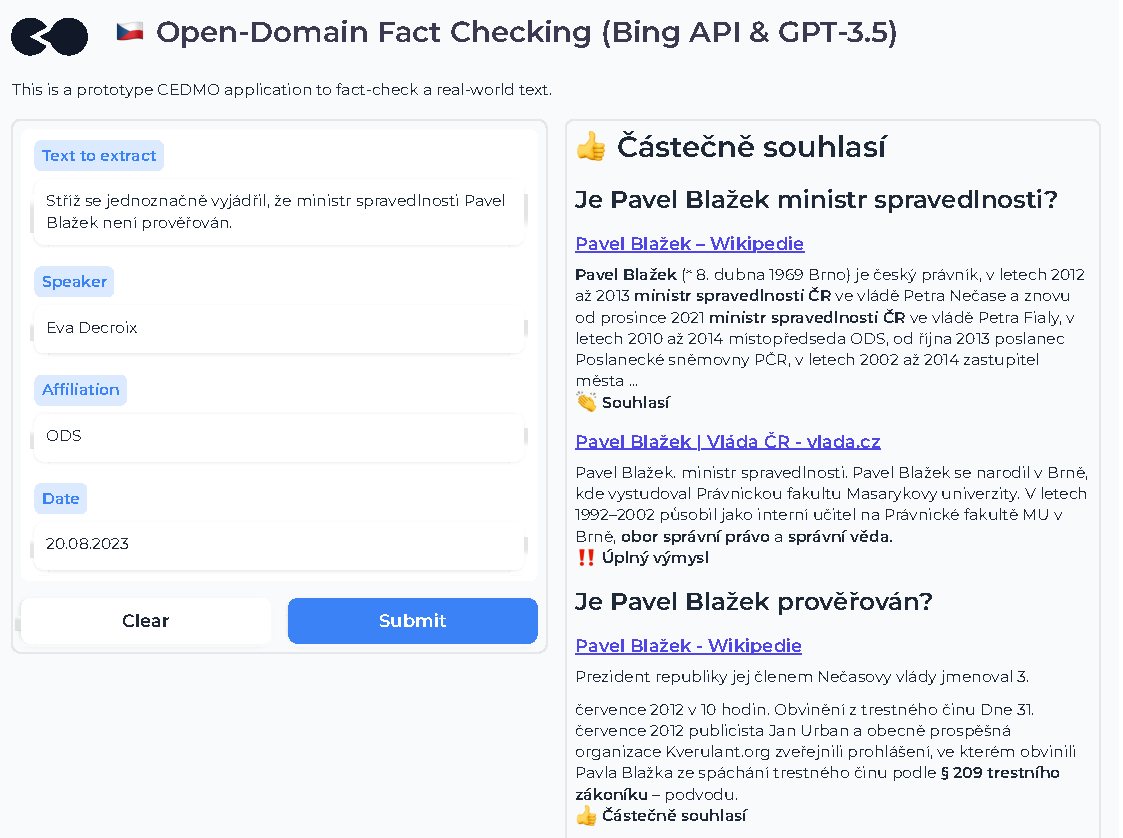
\includegraphics[width=14cm]{fig/bing.pdf}
    \caption{Proof-of-concept Czech fact-checking based on live-internet search (Bing API) and LLM prompting, based on the proposals of~\cite{bing} in Czech, using a real-world claim that was fact-checked by \href{https://demagog.cz/vyrok/22849}{\url{demagog.cz}} in June 2023}
    \label{fig:bing}
\end{figure}


\section{Claim generation}
\begin{itemize}
    \item Approches such as QACG exploit Question Answering
    \item The task of extreme summarization (XSum) focuses on summarizing a long body of text into a single sentence, focusing on its most relevant aspects and facts
    \item CLEF-CheckThat postulates the task of classifying \textit{Checkworthiness} of different parts of a long texts, such as a political debate
\end{itemize}

\section{NLP Generative task benchmarking}
\subsection{BERTScore}
\subsection{AlignScore}